% vim: set expandtab tabstop=4 shiftwidth=4 textwidth=80:

\documentclass{article}
\usepackage[inner=2.5cm,outer=2.5cm,bottom=1.8cm,top=1.8cm]{geometry}
\usepackage{graphicx}% Include figure files
\graphicspath{ {./graphics/} }
\usepackage{caption}
\usepackage{numprint} % rounds numbers in tables
\npdecimalsign{.}
\nprounddigits{5}
\captionsetup{justification=centering}
\usepackage{wrapfig}
\usepackage{tabu} % for changing individual row fonts
\usepackage{amssymb, amsmath}
\usepackage[mathscr]{euscript}
\usepackage{dsfont}

% nicely written chi
\def\Chi{\raisebox{2pt}{$\chi$}}

%% new column table for tabu to center paragraph cells
% http://tug.org/mail-archives/texhax/2007-March/008042.html
\usepackage{array}
\newcolumntype{C}{>{\centering\arraybackslash}m{2.8cm}} 

% to thicked table lines
\usepackage{booktabs}

% make rows in tables wider
\renewcommand{\arraystretch}{1.4}% Wider

\title{Improving Product Search with Session Re-Rank\\
    \large{a CS341 data mining project}}
\author{Charles Celerier (cceleri), Bill Chickering (bchick),
        and Jamie Irvine (jirvine)}

\begin{document}

\maketitle

Walmart.com maintains an online catalog of over 2M products. Consequently,
enabling users to quickly find products that conform to their specific needs and
tastes is especially challenging. Given the difficulty of its task,
Walmart.com's product search engine does an impressive job of interpretting the
user-provided query and rapidly returning relevant results. Yet, there remains
highly significant information that is not fully leveraged. The details of a
user's online shopping session are indicative of a user's intent and
compliment---indeed, provide context for---the user-provided query. In this
report we describe and analyze a ranking scheme we call {\em Session Re-Rank}
({\em SRR}) that can potentially induce a large increase in both
click-through-rates and conversions on the first page of query results.

\section{The Technique}\label{sec:technique}

{\em SRR} works by comparing previously clicked items with the top $N$ items
returned by the search engine in reponse to a query. Items in the top $N$ that
are sufficiently similar to previously clicked items are promoted. The extent
(i.e. number of positions) of the promotion for a particular item is a function
of its similarity to previously clicked items, its original position, and the
promotions of other items.

The similarity between an item to be shown and a previously clicked item is
determined within five distinct vector spaces: {\em click-space}, {\em
cart-space}, {\em query-space}, {\em title-space}, {\em item-space}. The
non-unique representation of an item within each of these spaces may be thought
of as a binary vector or a set of objects. (MapReduce jobs process historic
query data to construct indexes whose keys are itemids and values are lists of
the appropriate objects. Great care went into ensuring that index entries can be
accessed in $\mathcal{O}(1)$ and that two entries can be merged to compute their
intersection or union in linear time.) The similarity $J_s(A, B)$ of two items,
$A$ and $B$, within a particular space $s$ is determined using Jaccard
similarity. Similarities within particular spaces are then weighted and summed
to determine the composite similarity
\begin{equation}\label{eqn:similarity_metric}
    S(A, B) = \sum_s{C_s\cdot(J_s(A, B))^{\alpha_s}},
\end{equation}
where $C_s$ and $\alpha_s$ are tuning parameters. The score $\sigma$ attributed
to an item to be shown is then the summation of composite similarities between
itself and all previously clicked items plus the click-through-rate (CTR)
$\Gamma_i$ of the item's original position $i$
\begin{equation}\label{eqn:rerank_score}
    \sigma(A) = \sum_{B \in P}{S(A, B)} + \Gamma_i,
\end{equation}
where $P$ is the set of previously clicked items. 

Another important parameter of {\em SRR} is the insert position $I_0$, which
indicates that the top $I_0$ positions of the original ordering are to remain
fixed. For the results discussed in this report, we use $I_0 = 2$, meaning that
we never reorder the first two items of query results. We found this configuration
maximized our metrics, although, we suspect this may largely be due to users'
bias toward clicking on the first one or two positions indepedent of what is
shown there. That is, $I_0 = 0$ might prove optimal for an online implementation.

\section{Similarity Spaces}\label{sec:similarity_spaces}

The premise behind {\em click-space} is that two items are similar if they are
both clicked within the same online shopping session. The dimensions, or
objects, of this space are therefore past user-sessions. The {\em clicks-index}
for the data presented in this report was contructed using approximately half of
the provided data, or about 60M queries (about 120M page views).

{\em Cart-space} is based on the notion that two items are similar if they ever
appear in a shopping cart together. The objects of this space are therefore
shopping carts. The {\em clicks-index} for the data presented in this report was
also contructed using approximately half of the provided data.

Items are also considered similar if they appear in a query together. The
objects of {\em query-space} are therefore queries. We make a distinction,
however, between {\em user-queries} and {\em unique-queries}. The former are the
well-defined entities within the raw Walmart data. The latter is an abstraction
based on the notion that multiple {\em user-queries} can correspond to a single
{\em unique-query}. To derive {\em unique-queries} from our data, we cluster
{\em user-queries} according to following policy: two {\em user-queries} with the same search
attributes (e.g. category or price filters) are considered the same {\em
unique-query} if the strings constructed by concatenating the space-seperated,
stemmed (we use the Python stemming.porter2 module), and forced to lower-case terms
from each of their rawqueries are equal. We point out that while we achieved
better results with this policy compared to simply using {\em user-queries}, we
have no reason to believe that this is the ideal way to cluster queries for use
within {\em SRR}. Indeed, we believe one way to improve {\em SRR} is to optimize 
the query clustering policy.

{\em Title-space} is straightfoward. Each item is associated with a set of terms
from its title. We ignore case, but at present do not stem, discard stop words,
or weigh terms in any way. 

Finally, the structure of {\em item-space} is unique because it involves a level
of indirection. The premise here is that if items A and B are clicked in a
single user-session and items A and C are clicked in another user-session, that
items B and C are similar because they have item A in common. In this way, a
large number of relationships between items is created. {\em Item-space}
resembles {\em click-space} in that if two items are clicked during a single
session, they will have nonzero similarity. It differs from {\em click-space} in
two key respects, however. First, items that have historically never been
clicked in the same session can have nonzero similarity if they were each
clicked with a common third item. Second, if items are clicked together in many
sessions this will increase their Jaccard similarity in {\em click-space} but
not in {\em item-space}.

\section{An Example}


%\begin{wrapfigure}[4]{r}{0.1\textwidth}
%    \vspace{-10pt}
%    \centering
%    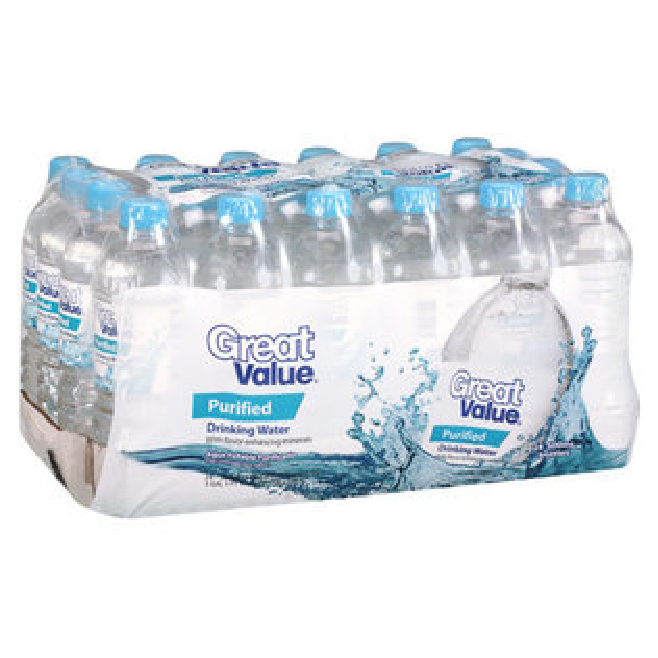
\includegraphics[width=0.1\textwidth]{bottled_water.eps}
%\end{wrapfigure}

%\begin{wrapfigure}[5]{l}{0.08\textwidth}
%    \vspace{-11pt}
%    \centering
%    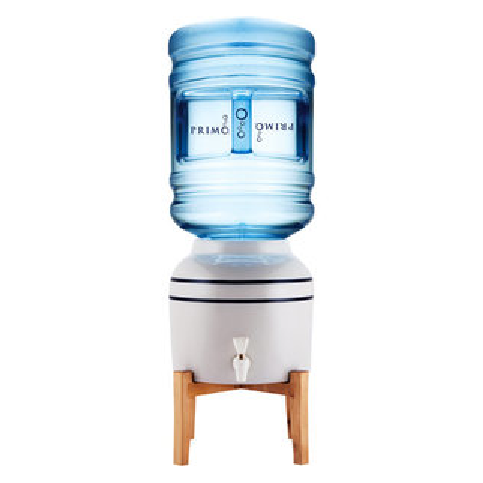
\includegraphics[width=0.1\textwidth]{water_cooler.eps}
%\end{wrapfigure}

%\begin{wrapfigure}[5]{r}{0.1\textwidth}
%    \vspace{-10pt}
%    \centering
%    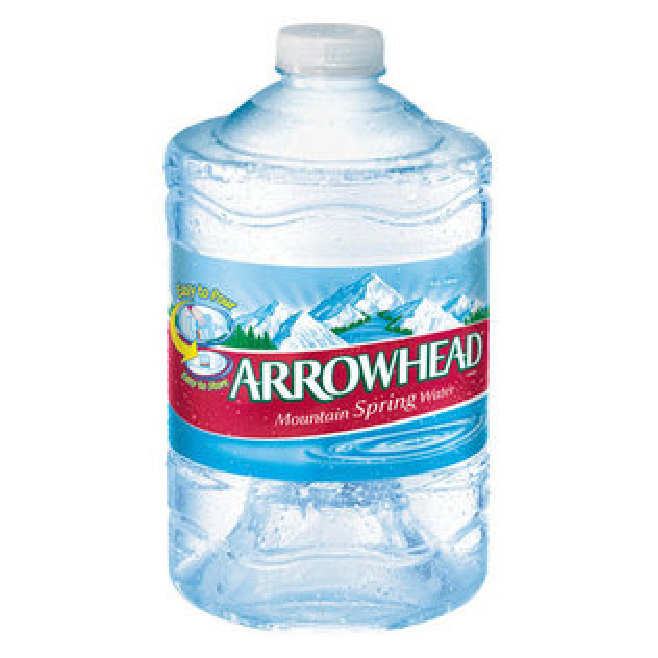
\includegraphics[width=0.1\textwidth]{arrowhead_water.eps}
%\end{wrapfigure}

To illustrate the efficacy of our technique, we present a real query example.
The only fictitious part of the example will be our shopper's name, David.
David is interested in the ``Primo Ceramic Crock Water Cooler with Stand'' and
clicks on this item during his session. Sometime later he navigates to the
``Grocery $\rightarrow $Beverages $\rightarrow $Water'' category and searches
for ``water''. He is presented with 300+ results and clicks the 90th item, a 3 liter
jug of water.

The top six original results are compared to the {\em SRR} results in Table
\ref{tab:compare_orderings} where the first and third column represent the
original ranking presented to David. Note that we rerank the 90th item from the
original results to be the 3rd item in the {\em SRR} results.
Tables \ref{tab:original_sim_scores} and \ref{tab:rerank_sim_scores} show the
similarity scores from each index for each item in the two orderings compared to
David's lone previously clicked item. In each of these tables, the first column
correponds to Table \ref{tab:compare_orderings} and the second column is the
similarity metric from Equation (\ref{eqn:similarity_metric}) using our
optimized tuning parameters.
\begin{table}[p!]
    \centering
    \begin{tabu}{m{.3cm} m{6cm} m{.45cm} m{7cm} }
        \rowfont{\bfseries} & Original Ordering & & {\em SRR} Ordering \\
        \toprule
        1. & Great Value Purified Water, 24ct         & 1.  & Great Value Purified Water, 24ct \\ \midrule
        2. & Nestle Waters Bottled Spring Water, 24ct & 2.  & Nestle Waters Bottled Spring Water, 24ct \\ \midrule
        3. & Voss Water, 16.9 oz (Pack of 24)         & 90. & Arrowhead Mountain Spring Water, 3 l \\ \midrule
        4. & CA Cherry Sparkling Water, 1 l, 12pk     & 63. & Great Value: Distilled Water, 1 Gal \\ \midrule
        5. & CA Water, 1 l, 12ct                      & 38. & Arrowhead Mountain Spring Water, 2.5gal \\ \midrule
        6. & CA Peach Sparkling Water, 1 l, 12ct      & 8.  & CA Orange Sparkling Water, 1 l, 12pk \\
        \bottomrule
    \end{tabu}
    \caption{Original Ordering vs. {\em SRR} Ordering for ``water'' query}
    \label{tab:compare_orderings}
\end{table}
\begin{table}[htbp!]
    \centering
    \begin{tabu}{ c n{1}{5} n{1}{5} n{1}{5} n{1}{5} n{1}{5} n{1}{5} n{1}{5} }
    \rowfont{\bfseries} & \multicolumn{1}{c}{\Large$\sigma$} & \multicolumn{1}{c}{CTR} & \multicolumn{1}{c}{Clicks} & \multicolumn{1}{c}{Items} & \multicolumn{1}{c}{Carts} & \multicolumn{1}{c}{Queries} & {Titles}  \\
        \toprule
        %% raw similarity scores
        %1. & 0.943746587049 & 0.0754 & 0.00227790432802 &  0.017955801105   &  0.0 &  0.0104712041885   &  0.0909090909091 \\ \midrule
        %2. & 1.20210752946  & 0.0390 & 0.00389105058366 &  0.0251450676983  &  0.0 &  0.0254833040422   &  0.0833333333333 \\ \midrule
        %3. & 0.357056025563 & 0.0254 & 0.0              &  0.0227882037534  &  0.0 & 0.00555212831585   &  0.0769230769231 \\ \midrule
        %4. & 0.75268102742  & 0.0195 & 0.0016835016835  &  0.0233918128655  &  0.0 &  0.0016339869281   &  0.0666666666667 \\ \midrule
        %5. & 0.736731785955 & 0.0153 & 0.00173310225303 &  0.016077170418   &  0.0 &  0.00390015600624  &  0.0666666666667 \\ \midrule
        %6. & 0.174834647629 & 0.0129 & 0.0              &  0.00954198473282 &  0.0 &  0.000793021411578 &  0.0666666666667 \\ \midrule
        
        % tuned scores
        1. & 0.943746587049 & 0.0754 & 0.525001355894 & 0.160481073286 & 0.0 & 0.153493353029 & 0.02937080484    \\ \midrule
        2. & 1.20210752946 & 0.039 & 0.686161147707 & 0.210098155039 & 0.0 & 0.239452362893 & 0.0273958638253    \\ \midrule
        3. & 0.357056025563 & 0.0254 & 0.0 & 0.194190538676 & 0.0 & 0.11176890762 & 0.0256965792667              \\ \midrule
        4. & 0.75268102742 & 0.0195 & 0.451335466924 & 0.198294695203 & 0.0 & 0.060633906259 & 0.0229169590345   \\ \midrule
        5. & 0.736731785955 & 0.0153 & 0.457935991834 & 0.146901991555 & 0.0 & 0.0936768435316 & 0.0229169590345 \\ \midrule
        6. & 0.174834647629 & 0.0129 & 0.0 & 0.0967767348166 & 0.0 & 0.0422409537777 & 0.0229169590345           \\
        \bottomrule
    \end{tabu}
    \caption{Index similarity scores of the top six original results to \\ ``Primo Ceramic Crock Water Cooler with Stand''}
    \label{tab:original_sim_scores}
\end{table}
\begin{table}[htbp!]
    \centering
    %\begin{tabu}{ c c  c }
    %    \rowfont{\bfseries} & CTR of demoted items & CTR of promoted items  \\
    %    \noalign{\smallskip}
    %    \noalign{\smallskip}
    %    \toprule
    %    {\bfseries \em SRR} & 6.24\% & 1.79\% \\
    %    \midrule
    %    {\bfseries \em RRR} & 2.42\% & 3.67\% \\
    %    \bottomrule
    %\end{tabu}
    \begin{tabu}{ c n{1}{5} n{1}{5} n{1}{5} n{1}{5} n{1}{5} n{1}{5} n{1}{5}}
    \rowfont{\bfseries} & \multicolumn{1}{c}{\Large$\sigma$} & \multicolumn{1}{c}{CTR} & \multicolumn{1}{c}{Clicks} & \multicolumn{1}{c}{Items} & \multicolumn{1}{c}{Carts} & \multicolumn{1}{c}{Queries} & {Titles}  \\
        \toprule
        %% raw similarity scores
        %1.  & 0.943746587049 & 0.0754     & 0.00227790432802 &  0.017955801105 &  0.0 &  0.0104712041885 &  0.0909090909091  \\ \midrule
        %2.  & 1.20210752946  & 0.0390     & 0.00389105058366 &  0.0251450676983 &  0.0 &  0.0254833040422 &  0.0833333333333 \\ \midrule
        %90. & 0.95310150677  & 0.00022623 & 0.00357142857143 &  0.027027027027 &  0.0 &  0.000920810313076 &  0.0833333333333\\ \midrule
        %63. & 0.949541641831 & 0.00049366 & 0.00261096605744 &  0.0338345864662 &  0.0 &  0.00385802469136 &  0.0833333333333\\ \midrule
        %38. & 0.93768536446  & 0.000914   & 0.00344234079174 &  0.0331384015595 &  0.0 &  0.0 &  0.0909090909091             \\ \midrule
        %8. & 0.896706599209 & 0.01       & 0.00355239786856 &  0.0248565965583 &  0.0 &  0.0 &  0.0666666666667             \\ \midrule

        % tuned scores
        1. & 0.944 & 0.0754   & 0.525 & 0.16  & 0.0 & 0.153  & 0.02947080484  \\ \midrule
        2. & 1.2   & 0.039    & 0.686 & 0.21  & 0.0 & 0.239  & 0.0274253      \\ \midrule
        3. & 0.953 & 0.000226 & 0.657 & 0.223 & 0.0 & 0.0455 & 0.027438253    \\ \midrule
        4. & 0.95  & 0.000493 & 0.562 & 0.266 & 0.0 & 0.0932 & 0.027458638253 \\ \midrule
        5. & 0.938 & 0.000914 & 0.645 & 0.262 & 0.0 & 0.0    & 0.0294         \\ \midrule
        6. & 0.897 & 0.01     & 0.656 & 0.208 & 0.0 & 0.0    & 0.0229         \\
        \bottomrule
    \end{tabu}
    \caption{Index similarity scores of the top six {\em SRR} results to \\ ``Primo Ceramic Crock Water Cooler with Stand''}
    \label{tab:rerank_sim_scores}
\end{table} 

The similarity scores from {\em title-space} are easily calculated by hand. We
will show the calculation for the {\em item-space} similarity for the 90th item
in the original ranking. By referring to the corresponding index for {\em
item-space}, we can recall that the 90th item was clicked in a same session with
39 different items and the previously clicked item was clicked in a same session
with 455 different items. The titles of the 13 items found in common are:
\begin{itemize}
    \item[] Great Value: Distilled Water, 1 Gal
    \item[] Nestle Waters Bottled Spring Water, 24ct
    \item[] Primo Mineral Water, 5 gal
    \item[] Deer Park Sumo Bottle Natural Spring Water, 3l
    \item[] Arrowhead Mountain Spring Water, 3l
    \item[] PUR Advanced Faucet Water Filter Vertical - Chrome
    \item[] Ozarka Natural Spring Water
    \item[] Formula 409 All Purpose Lemon Scented Cleaner, 32 fl oz
    \item[] Great Value Spring Water, 1 gal
    \item[] Nestle Pure Life Purified Water, .5l, 35pk
    \item[] Arrowhead Mountain Spring Water, 2.5gal
    \item[] Primo Ceramic Crock Water Cooler with Stand
    \item[] Augason Farms Emergency Water Storage Kit
\end{itemize}
We then calculate the similarity of the 90th item and the previously clicked
item in {\em item-space} to be $13/(455+39-13)=0.0270$.

We believe this example illustrates how our technique can form subtle
relationships between items based on historical user session data. In this case,
we have a shopper who had an interest in a water cooler and subsequently made a
query for ``water''. If the shopper had been in a brick-and-mortar store, he
likely would have been directed to the section of the store selling water jugs
to use with the cooler he had picked up. In this case, {\em SRR} recognized
David's previous click on a water cooler, related that water cooler to large
water jugs, and showed David the water jug he was looking for all along.

\section{The Data}

Walmart.com has generously supplied us with a large dataset consisting of about
250M pageviews comprising about 120M query results which occurred over about 30
days. The data includes the user-provided rawqueries together with search
attributes, visitorIds and sessionIds, shown items, clicked items, which items
were placed in a shopping cart, and which items were ultimately purchased. In
addition, they have provided detailed item information including title,
description, category, and other details. The query data was randomized with
respect to search time and then segregated into three disjoint sets. The first
set, which consists of about half of the data, was re-structured into indexes
that form four of the similarity spaces ({\em click-space}, {\em cart-space},
{\em query-space}, and {\em item-space}) we use to identify relationships
between items in realtime (the remaining similarity space, {\em title-space},
was compiled separately using the provided item data). The second set, which
consists of less than 5\% of the data, was used for testing and optimization,
allowing us to refine our technique and tune its parameters. And the third set,
which includes about 10\% of the data, was used in the experiments described and
analyzed in this report.

\section{The Technique vs The Experiment}

An important distinction should be made between the {\em SRR} technique and the
experiment described in this report. Both the technique and the experiment
leverage the provided data---however, the experiment is a simulation and a
limited one at that. A key limitation is that the provided query data is
confined to what the user was actually shown. That is, the search engine may
have identified several pages worth of results in response to a {\em
user-query}, but our dataset consists only of those pages actually seen by the
user.  Meanwhile, the concept behind the {\em SRR} technique calls for a search
engine to deliver to the algorithm the top $N$ items in response to a {\em
user-query} {\em independent of the number of items ultimately shown to the
user}. As a consequence, it is difficult, if not impossible, to simulate our
technique using shown query results that are truncated because a user only
viewed one or two pages.  Even more generally, the use of historic data to
demonstrate the consequences of a online ranking algorithm is intrinsically
limited by the fact that one cannot be certain how users would have behaved if
presented with different results. Nonetheless, we have done our best to conduct
the most fair and informative experiment and analysis.

\section{The Experiment}\label{sec:experiment}
A key feature of {\em SRR} is that it can only re-rank the results of a query if
a user has previously clicked on an item during an online session.
Consequently, {\em SRR} can only affect the subset of queries that occur in a
session with previous clicks. We denote this subset of queries as $\zeta$ and
limit our experiment and analysis to this set. It turns out that 25\% of all
queries are in $\zeta$. Moreover, 28\% of all clicks and 36\% of all purchases
occur within the query resultsets of $\zeta$, since there is a correlation
between previous clicks and clicks/purchases in a query.  Thus an impact to this
subset can have a significant impact overall.

The goal for the experiment is to simulate {\em SRR} using the provided
historical query data, which is limited to what users were actually shown. An
online implementation of our technique would receive the top $N$ items from the
search engine and re-rank them prior to showing any results to a user. Because
of this, the final ranking would be independent of the total number of items
actually seen by a user (determined by the number of pages a user clicked
through).  Our test set $\Chi$ therefore consists solely of queries within
$\zeta$ where either all items in the query resultset or at least $N=100$ items
were shown to the user. For example, if a user stops searching after viewing
only the 16 items on the first page (the default number of items on the first
page), this query is not included in $\Chi$, since it is unknown which other
items would have been considered for re-ranking. On the other hand, if the
search engine found only 13 items in response to a query,  we have the complete
query resultset and can therefore determine how {\em SRR} would have reordered
the shown items. Similarly, if more than $N=100$ were shown to the user, we can
determine the reordering regardless of whether the query resultset is truncated
since {\em SRR} only considers and re-ranks the first $N=100$ items. $\Chi$
makes up 30\% of $\zeta$, accounting for a total of 7.5\% of all queries.

\begin{figure}[htbp!]
    \centering
    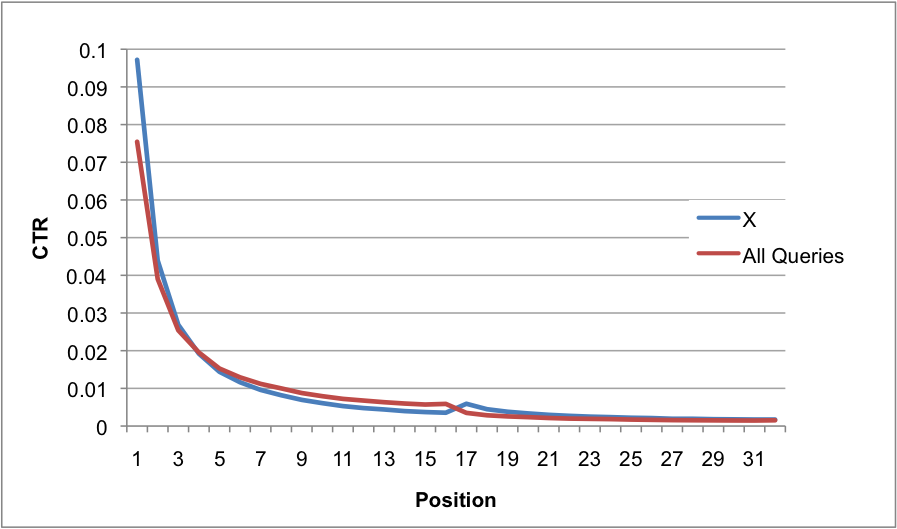
\includegraphics[width=\textwidth]{CTRcompare.png}
    \protect\caption{CTR as a function of position from the original data (i.e.
    not re-ranked) for the test set \protect\raisebox{2pt}{$\chi$} (blue) and
    all queries (red).}
    \label{fig:ctr_vs_position}
\end{figure}

To construct $\Chi$ we  must discard all queries with a number of shown results
less than $N=100$ that are also divisible by 16. The reason for this is that
Walmart.com provides two options for the number of items shown per page: 16 or
32. Thus, by performing the experiment on this subset of the data we precluded
queries where the top $N$ items are not available to our algorithm.  The choice
of $N=100$, meanwhile, is somewhat arbitrary and was made by balancing our
desire for a large test set with our desire to use a value appropriately large
for an online implementation. It is therefore quite possible that a larger value
of $N$ (e.g. 1000) would achieve better results in the actual online scenario.

While we must constrain $\Chi$ in this way due to the nature of the available
data, we stress that this subset is certainly biased with respect to queries in
general. For starters, queries with short resultsets are more likely to have all
of their resultset seen by a user, and therefore, are more likely to be included
in $\Chi$. It is not clear, however, if this particular bias tends to under- or
overestimate the effectiveness of {\em SRR} since, as we will show, {\em SRR} is
more effective on longer query results. Similarly, highly qualified
queries---e.g. through the use of category or price filters---tend to have
shorter resultsets, and hence, are more likely to be included in $\Chi$.

Just as interesting are the ways in which the queries and resultsets of $\Chi$
are not biased. In Fig. \ref{fig:ctr_vs_position} we show click-through-rate
(CTR) as a function of position of the original data (i.e. not re-ranked) for
both $\Chi$ and query results in general. The two curves shown in the figure are
quite similar, indicating that the quantity and distribution of clicks within
$\Chi$ are essentially representative of those in general. A few other features
of this figure warrant brief comment. First, we see that $\Chi$ has a larger CTR
for the top two positions. This is likely due to the fact that highly qualified
queries, which have shorter results and higher CTRs,  make up a higher
proportion of $\Chi$ than queries in general. While this difference does results
in a slightly higher frequency of clicks in $\Chi$, we have no reason to believe
that this alone results in a significant bias. Next, we see in the red curve a
discontinuity appears at position 17 as a result of the pagebreak. In the entire
dataset, the majoriy of queries are truncated at the first page, leading to
significantly fewer views of items on other pages and thus fewer clicks. This
discontinuity is absent from the blue curve since $\Chi$ has a less severe
dropoff in viewership from one page to the next.  The bump at position 17 can be
ascribe to users' tendency to disproportionately click on the topmost item shown
on a page. Indeed, if we normalize for number of pages viewed by a user, we see
this bump at 17 in the overal dataset as well. Consistent with this analysis, we
find another smaller drop in the red curve and smaller bump in the blue at
position 33.

\section{Metrics}

A true test of the effectiveness of {\em SRR} would require online A/B
testing. In the meantime, we can simulate the effect of {\em SSR} by running it
on historical data and examining the new positions of clicked and purchased items.
Assuming the user would have clicked or purchased the same items in this new ordering, 
we can compare the distribution of clicks in the original ranking to that yielded 
by {\em SRR}.

To compare two rankings of shown items, we focus on three key metrics. Our primary 
metric is the first-page CTR $\mathscr{C}$, defined as the likelihood that an item 
presented on the first page receives a click. Special attention to the first page is
reasonable, since 77\% of all queries 
are only one page long. This shows the importance of bringing desirable items to the 
first page and it motivates our focus on $\mathscr{C}$. We calculate this metric by 
counting the number of items in first-page positions that were clicked and dividing 
by the number of total items in first-page positions. More formally
\begin{equation}
    \mathscr{C} = \frac{\sum_{q \in Q}\sum_{i=1}^{L_q}\mathds{1}\left\{click\; @\; i \wedge i \leq 16\right\}}{\sum_{q \in Q}\sum_{i=1}^{L_q}\mathds{1}\left\{i \leq 16\right\}},
\end{equation}
where $Q$ is a set of query results, $L_q$ is the number of results for query $q$, and
the number 16 is due to the fact that 16 items are shown on a page.

Our second metric is the purchasing rate of items on the first page $\mathscr{P}$. This is 
similar to $\mathscr{C}$, except here we consider purchases per first-page item 
instead of clicks. It is calculated as the number of items in first-page positions that 
were purchased divided by the total number of items in first-page positions. The 
importance of position for purchases is even stronger than that for clicks. While 76\% of 
all clicks were presented on the first page, that number is 88\% for purchases. Formally,
we have
\begin{equation}
    \mathscr{P} = \frac{\sum_{q \in Q}\sum_{i=1}^{L_q}\mathds{1}\left\{purchase\; @\; i \wedge i \leq 16\right\}}{\sum_{q \in Q}\sum_{i=1}^{L_q}\mathds{1}\left\{i \leq 16\right\}}.
\end{equation}

The first two metrics focus on whether or not a desirable item was presented on the 
first page. To obtain a more granular picture of where desirable items are positioned, 
we also compute a third metric which we call {\em click-position score} $\mathscr{S}$. 
Somewhat similar to normalized discounted cumulative gain (NDCG), which is a common metric
of search engine results, this score weighs the value of a clicked item by its position, 
giving higher weights to items closer to the top. For $\mathscr{S}$, the weight given to 
a click in position $i$ is the CTR at position i $\Gamma_i$. In this way, we equate how 
often users click on a certain position to how valuable it is to put a desirable 
item there. Formally, we define {\em click-position score} as
\begin{equation}
    \mathscr{S} = \frac{1}{\left\vert{Q}\right\vert}\sum_{q \in Q}\sum_{i=1}^{L_q}\mathds{1}\left\{click\; @\; i\right\}\Gamma_i.
\end{equation}

These metrics give a sense of how successful a ranking scheme is. Each one looks at a slightly 
different aspect of the ordering. Indeed, optimizing for one metric does not necessarily 
optimize for the others. We focus our optimizations and primary analysis on $\mathscr{C}$
as we believe it is the simplest and has the clearest impact to overall CTRs.

\section{Results}

Figure \ref{fig:avg_clicks_position_score} shows the clicks-position score
$\mathscr{S}$ as a function of each of the coefficients $C_s$ discussed in
sections \ref{sec:technique} and \ref{sec:similarity_spaces}. Here, we vary a
single coefficient, corresponding to one of the five similarity spaces---{\em
click-space}, {\em cart-space}, {\em query-space}, {\em title-space}, or {\em
item-space}---while setting the others to zero. The ranking score for each of
the top $N=100$ items is then determined by only two terms, as per Eqs.
\ref{eqn:similarity_metric} and \ref{eqn:rerank_score}, as
\begin{equation}\label{eqn:single_coeff_score} 
    \sigma(A) = \sum_{B \in P}{C_s\cdot(J_s(A,B))^{\alpha_s}} + \Gamma_i, 
\end{equation}
where, as before, $P$ is the set of previously clicked items and $\Gamma_i$ is
the CTR of the original position of item $A$. (Note that the exponents
$\alpha_s$ are held fixed during these measurements.) Thus, since $\Gamma_i$ is
a monotonically decreasing function of position $i$, when $C_s = 0$, {\em SRR}
returns the original ordering.

In each case, as $C_s$ is increased from zero, the degree of reordering is
enhanced.  And for each coefficient, this reordering is accompanied by an
increase in $\mathscr{S}$ indicating a greater concentration of clicked items,
on average, in the top positions of query results as compared to the original
ordering.  Moreover, with the exception of {\em title-space}, the score
increases monotonically with each coefficient. In the case of {\em
title-space}, a broad maximum can be seen around $C_s = 0.05$. This indicates
that an optimal combination between the contributions from {\em title-space}
and CTRs exists, which maximizes $\mathscr{S}$. For all other coefficients,
however, a maximum cannot be found. Rather, the value of $\mathscr{S}$
asymptotically increases with value of $C_s$, which demonstrates that the
optimal average ordering, according to the metric $\mathscr{S}$, is determined
solely by the similarity space irrespective of the original ordering.

\begin{figure}[htbp!]
    \centering
    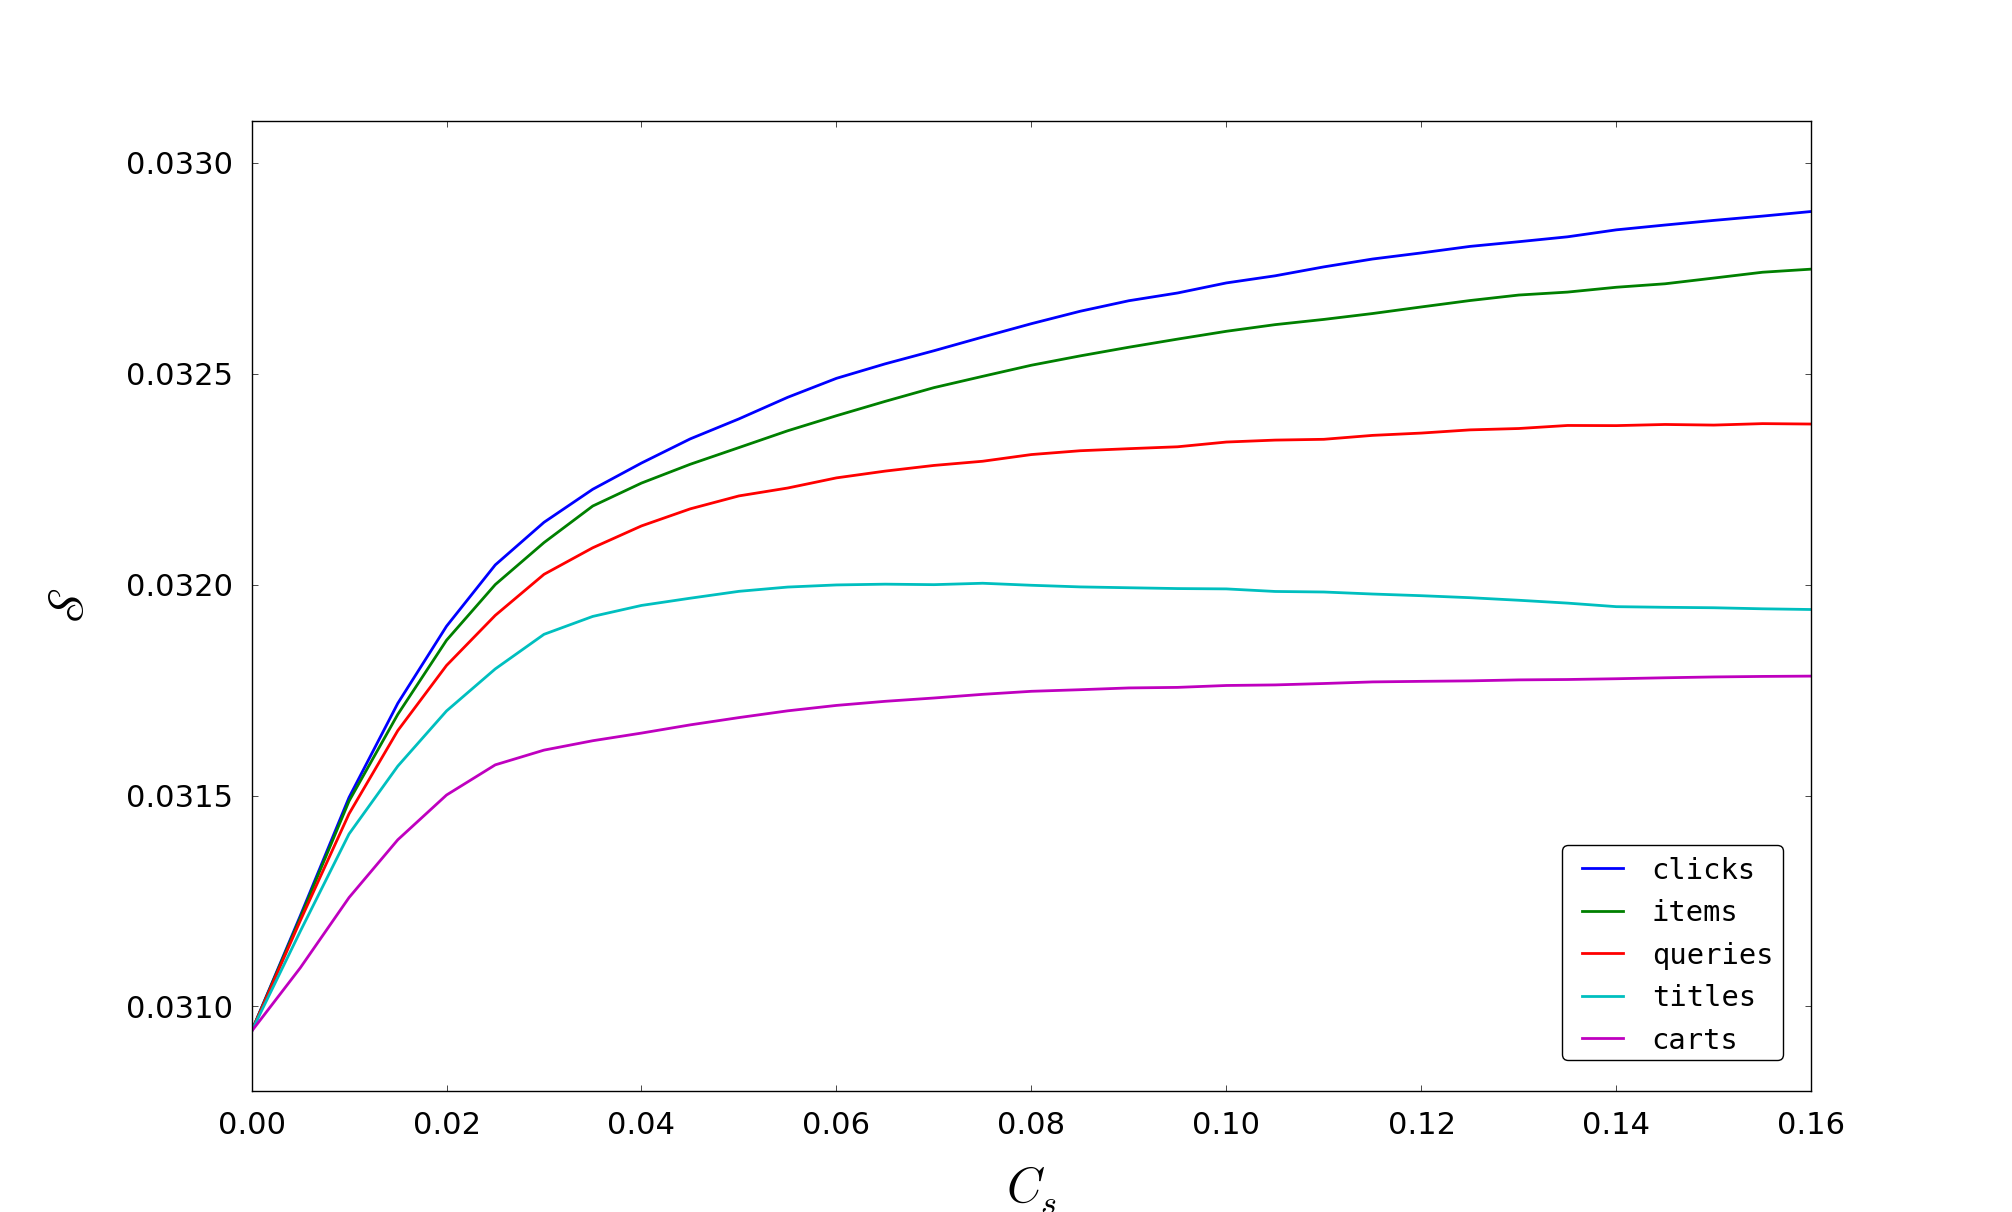
\includegraphics[width=\textwidth]{000050_0_48chunk_k100_i2_n100_avg_click_position_score_0-0_16.png}
    \caption{Clicks-position score $\mathscr{S}$ as a function of individual similarity space coefficients $C_s$. For each curve, a single coefficient is varied with all other set to zero.}
    \label{fig:avg_clicks_position_score}
\end{figure}

We employ hueristics to manually optimize the coefficients $C_s$ and exponents
$\alpha_s$, which are outside the scope of this report. We do want to emphasize
two important points regarding this optimization, however. First, as previously
mentioned, we conduct this optimization on a set of data that is both disjoint
with that used to construct the similarity spaces indexes and with that used to
conduct the experiment whose results are shared below. Second, we find that the
optimal configuration includes nonzero values for all five coefficients showing
that their contributions are not fully redundant.

With our optimized combination of coefficients we find that {\em SRR}
significantly outperforms the original ordering on queries in $\Chi$. As shown
in Fig.  \ref{fig:compare_metric_performance}, the re-ranking achieves a 16.9\%
increase in $\mathscr{C}$ compared to the original ordering. The implication is
that items on the first page of the re-ranking are 16.9\% more likely to be
clicked than those in the original ordering. With over 2M queries in our test set
$\Chi$, these results are statistically significant, producing a 95\%
confidence interval of [16.4\%, 17.4\%] for $\mathscr{C}$.

\begin{figure}[htbp!]
    \centering
    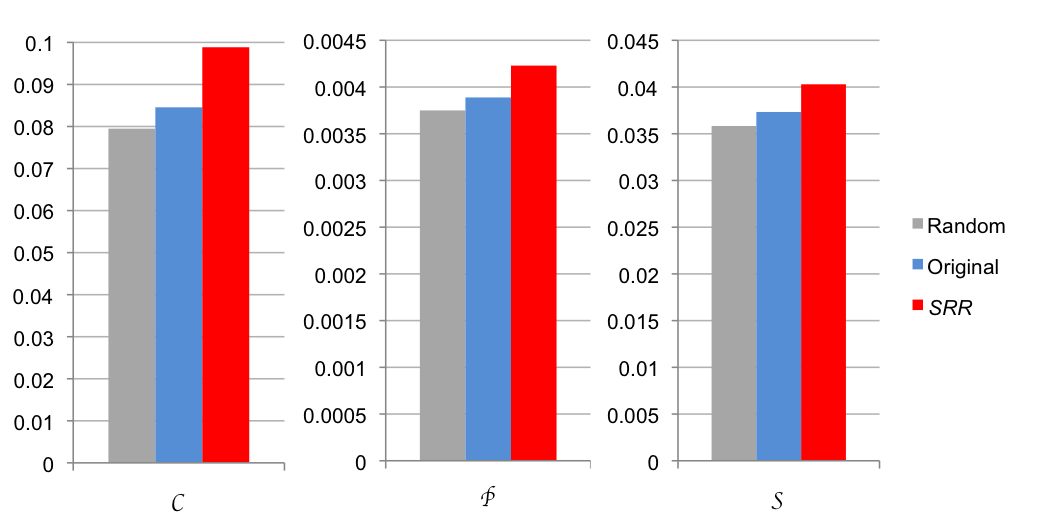
\includegraphics[width=\textwidth]{moneyshot.png}
    \caption{Comparison of the original ranking (blue) to that of randomly re-ranking (grey) and {\em SRR} (blue) using all three metrics: front-page CTR $\mathscr{C}$, front-page purchase rate $\mathscr{P}$, and click-position score $\mathscr{S}$.}
    \label{fig:compare_metric_performance}
\end{figure}

Notably, we see these results despite the benefit the original ranking receives
from "position bias", the well-established phenomenon that users tend to click
on items presented at the top of a list. Figure \ref{fig:ctr_vs_position} shows
how dramatically more likely Walmart.com users are to click on items positioned
near the top. It seems reasonable to suppose that "position bias" contributes
to this distribution of CTRs. We compensate for the large CTR of the first two
positions by setting the insert position $I_0 = 2$ such that the top two items
remained fixed. While this does improve the metrics for {\em SRR}, we emphasize
that choosing $I_0 = 0$ would not qualitatively change our results. Another
obstacle overcome by {\em SRR} is that there is little room for improvement in
first-page CTR, since the majority of clicks in $\Chi$ (58\%) are already
on the first page.

To ensure that these results are not due to an underlying structure of the
data, we constructed a Random Re-Ranker {\em RRR}. {\em RRR} operates exactly
as {\em SRR} does, except instead of calculating various similarity scores, it
uniformly chooses at random a number between 0 and 1. This randomized algorithm
significantly hurts the results in all three metrics, suggesting that {\em SRR}
achieves its success by intelligently deciding which items are more likely to
be clicked. 

Indeed, Table \ref{tab:promote_demote_table} compares the average
CTR of items {\em SRR} moves on or off the first page to those chosen randomly. 
By accurately determining a user’s preference for certain items, {\em SRR} promotes items with a
significantly higher CTR than it would by blindly picking items from other pages. 
Similarly, it demotes first-page items with a lower CTR than an average item on
the first page. With these successful decisions, {\em SRR} manages to outperform the original
ordering in the face of a number of disadvantages.

\begin{table}[htbp!]
    \centering
    \begin{tabu}{ c c  c }
        \rowfont{\bfseries} & \multicolumn{1}{C}{CTR of promoted items} & \multicolumn{1}{C}{CTR of demoted items}  \\
        \noalign{\smallskip}
        \noalign{\smallskip}
        \toprule
        {\bfseries \em SRR} & 6.24\% & 1.79\% \\
        \midrule
        {\bfseries \em RRR} & 2.42\% & 3.67\% \\
        \bottomrule
    \end{tabu}
    \caption{CTR of items promoted to the first page and demoted off the first
    page. {\em SRR} siginificantly outperforms random re-ranking in both categories.}
    \label{tab:promote_demote_table}
\end{table} 

Taking a closer look, we see that the performance of {\em SRR} is correlated to
query length $L_q$. Figure \ref{fig:click_position_score_vs_query_length} shows
the percent increase in $\mathscr{S}$ as a function of $L_q$. While it on
average outperforms the original ordering for query results of any length, it
gains greater improvement as $L_q$ increases.  This is an impressive feature of
{\em SRR}, since as $L_q$ increases, the density of clicked items decreases
making them more difficult to select. At the same time, longer results provide
greater opportunity for improved ranking, which {\em SRR} successfully exploits
as shown by the data.

The specific trends within the data are more difficult to understand. There appear
to be linear trends for $L_q \in [1,16]$ and $L_q \in [17,32]$, which
correspond to single and double page results, respectively. Meanwhile, the
trend for $L_q > 32$, while generally increasing, is less clear. We speculate
that these trends are due to idiosyncrasies in user behavior but details remain
unclear to us.

\begin{figure}[htbp!]
    \centering
    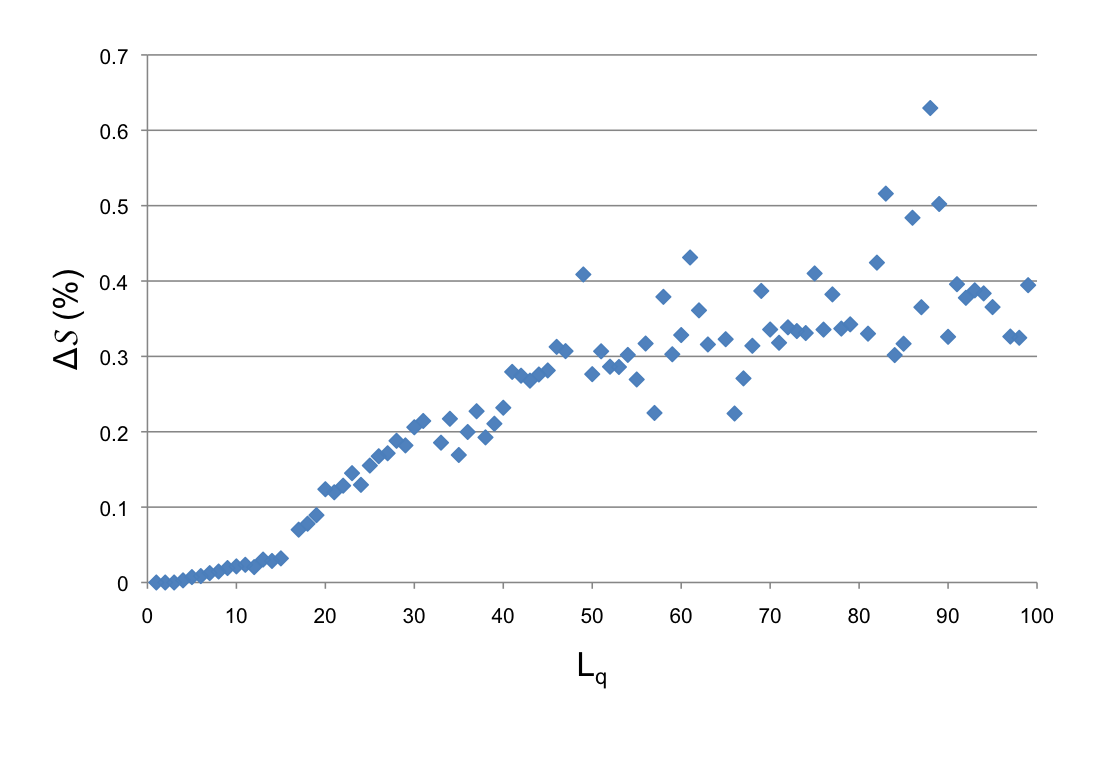
\includegraphics[width=\textwidth]{scorebylen.png}
    \caption{Change in click-position score $\mathscr{S}$ as a function of query length $L_q$.}
    \label{fig:click_position_score_vs_query_length}
\end{figure}

\section{Discussion}

We have established that {\em SRR} significantly improves the ordering
of search results by all three metrics on the dataset $\Chi$. Note that $\Chi$
represents 30\% of $\zeta$ while the remaining 70\% of queries were truncated
short. We call this set of truncated queries, $\tau$. As discussed in Section 6, 
we cannot accurately test {\em SRR} on $\tau$ since it would have performed 
differently on this set of queries.\footnote{We ran {\em SRR} on all of {\zeta},
treating truncated queries as complete ones of the length shown to the user. The
results were similar to those of {\Chi} and in some metrics better:
{\Delta}$\mathscr{C}$ = 12.5\%, {\Delta}$\mathscr{P}$ = 8.7\%, and
{\Delta}$\mathscr{C}$ = 8.2\%. We omitted these results from the main paper
because we feel that testing on all queries in {\zeta} is not a representative
experiment.}

Extrapolating from $\Chi$ to $\tau$ is difficult since, the characteristics of
the two sets are inherently different, potentially introducing biases that
affect {\em SRR}'s performance. For instance, queries in $\Chi$ are ones in
which the user search to the end or through at least $N=100$ itesm, potentially
indicating disinterest in the first page results and favoring any reordering. On
the other hand, queries in $\Chi$ are on average shorter than those in $\tau$
and, as suggested by Figure \ref{fig:click_position_score_vs_query_length}, {\em SRR}
performs better on longer queries. 

While it is unclear whether {\em SRR} would do better or worse on $\tau$, we can
infer a very loose lower bound on $\mathscr{C}$ over all of $\zeta$ by assuming
that {\em SRR} performs as badly as it reasonably coult on $\tau$. When run on
$\Chi$, {\em SRR} on average demotes 8\% of all first-page clicks, but replaces
them with even more clicks from other pages. In the worst case, we assume that
when run $\tau$, it would demote 8\% of first-page clicks but replace them with
0 clicks from other pages. Assuming this pessimistic lower bound for the 75\% of 
queries in $\zeta$ that make up $\tau$, {\em SRR} would still sligthly
outperform the original ordering across all queries (+0.01\%).

If instead we assume that {\em SRR} would perform similarly on $\tau$
as it does on $\Chi$, we can get a more realistic estimate of the impact that the
algorithm would have overall. Broadening the scope of our results to all
queries (even those outside of $\zeta$ which re-ranker could not impact), 
we get an overall increase in $\mathscr{C}$ by 4.5\% and an overall increase in $\mathscr{P}$
by 3.0\%. To get a better sense of what
this impact means, consider the set of purchases that occur in the
first page. Increasing the purchasing rate for these items by 3\% would
increase the absolute size of this set by 3\%. Since this set
comprises 88\% of all purchases, increasing it by 3\% would increase
the total number of purchases on the website overall by 2.6\%, which
is a significant increase for a search engine on the scale of Walmart’s.

\end{document}

